\section{Aufgabe Team 4}\label{sec:04_01_aufgabe}
(Autorin: Jennifer Vormann)\\
\begin{figure}
  \begin{center}
    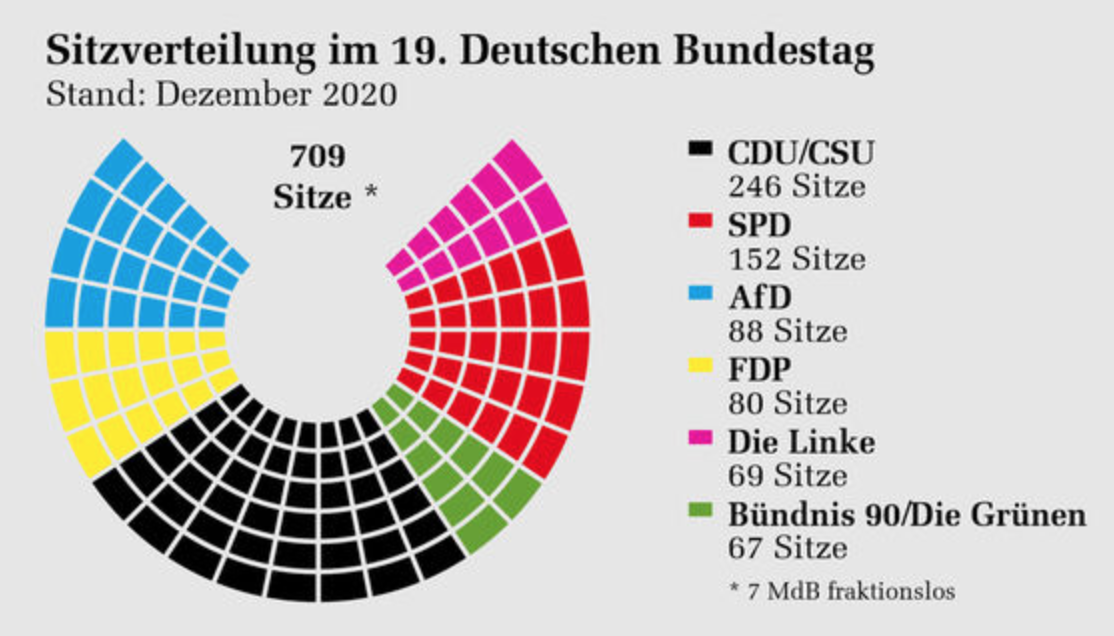
\includegraphics[width=0.8\textwidth]{Dokumentation-main-2/main_document/chapters/05-Interaktion-Abgeord/sitzverteilung_19wp_bild.jpg}
  \end{center}
  \caption{Sitzverteilung im 19. Deutschen Bundestag \cite{sitze19Bundestag}}
  \label{fig:sitzverteilung}
\end{figure}
\\
\textbf{Team} \\
Rico Stucke | Florian Thom | Jennifer Vormann\\
\\
\textbf{Thema}\\
Graph-basiertes Informationssystem zur Analyse sozialer Interaktion im Deutschen Bundestag\\
\\
\textbf{Aufgabe von Team 4}\\
Unsere Aufgabe bestand darin, die Beziehungen zwischen Abgeordneten darzustellen. Die Beziehungen ausgehend von Abgeordneten zu einer Fraktion und von einer Fraktion zu einem Abgeordneten wurden ebenso einbezogen und betrachtet. Kommentare von einer Fraktion zu einer anderen wurden bei dieser Teilaufgabe außen vor gelassen, da dies Aufgabe von Gruppe 5 war. \\
In der Praxis bedeutete das für uns Daten zwischen unterschiedlichen Datenbanken und Servern zu verarbeiten und zu übertragen. Ziel war es, eine Graphdatenbank zu haben, in der die Interaktionen zwischen den Abgeordneten während der Bundestagssitzungen ersichtlich sind und abgerufen werden können. Es wurden alle Sitzungstage der 19. Wahlperiode betrachtet. Aktuell fanden in dieser Wahlperiode über 200 Sitzungstage statt. Wechsel von Abgeordneten in eine andere Fraktion wurden vorerst außen vor gelassen. Das genaue Vorgehen zur Erreichung dieses Ziels wird im nachfolgenden Kapitel erläutert. Der Hintergrund ist, herauszufinden, ob der Ton im Bundestag tatsächlich rauer geworden ist. Für die Analyse liegen die entsprechenden Sitzungsprotokolle als XML-Dateien vor. Uns wurde von Team 3 Zugang zu einer MongoDB mit den bereits bereits gespeicherten Daten gewährt.
\section{Vorgehen}\label{sec:04_02_vorgehen}
\noindent
(Autorin: Jennifer Vormann)
\subsection{Absprachen}
Im Rahmen der Plenarsitzungen wurde mit allen Gruppen gemeinsam das Vorgehen besprochen. Dies geschah im Rahmen der wöchentlichen Meetings. Zusätzlich fanden diverse Absprachen mit Team 2 und 3 statt. Es musste geklärt werden, wann wir die ersten Daten erhalten und in welcher Form. Mit Team 5 musste abgesprochen werden, ob wir den gleichen Server und/oder die gleiche Datenbank benutzen wollen. Hier wurde sich in beiden Punkten dagegen entschieden. Die Kommunikation mit Team 7 fand ebenfalls ergänzend statt, um die Weiterleitung der Daten zu besprechen.
\subsection{Planung \& Setup}
Zu Beginn des Projektes haben wir ein GitHub Repository erstellt und den virtuellen Server aufgesetzt. Wir haben einen Zeitplan angefertigt und eine Planungspräsentation vorbereitet, die auch anschließend in der Plenarsitzung gehalten wurde. Im Team haben wir uns gemeinsam auf ein Datenbankschema festgelegt. Das Datenbankschema wird im Unterkapitel zum Entwurf näher erläutert.\\
\\
Nachfolgend verständigten wir uns im Team und auch mit Gruppe 5 zu den Technologien und nahmen die entsprechenden Installationen vor. Wir entschieden uns für die Graphdatenbank Neo4j, um die Beziehungen zwischen den Abgeordneten gut visualisieren zu können. Eine weitere Intention war die Lust Neo4j und Cypher neu zu erlernen. Beim Skript entschieden wir uns für ein Python Skript. Das Skript, welches zu implementieren war, sollte eine Verbindung zu den Datenbanken (MongoDB, Neo4j) aufbauen und die Daten einzeln von der MongoDB einlesen. Anschließend sollte es in der Lage sein, die Daten umzuformen - in Nodes, Properties & Relationships. Als letzter Schritt sollte die Sicherung in die Graphdatenbank Neo4j realisiert werden, um die Daten Gruppe 7 zur Verfügung stellen zu können. Zum Ende unseres Projektes haben die gesamte Umsetzung inklusive Ergebnissen und Ausblick in dieser Dokumentation zusammengetragen. Die Abschlusspräsentation wurde erstellt und vor dem Kurs gehalten.
\section{Entwurf}
(Autor: Florian Thom)
\newline
\newline
Mit diesem Unterkapitel werden Hintergrundwissen, Überlegungen und Prozesse zur Umwandlung von unstrukturierten Daten aus einer NoSQL-Daten\-bank in ein graphenoptimiertes Schema zur Darstellung gegebener Interaktionen zwischen Abgeordneten des Bundestages präsentiert.
\subsection{Überblick}
Diese Arbeit setzt ein Basisverständnis von Graphdatenbanksystemen voraus. Dementsprechend werden zu besagten Graphdatenbanken keine Begriffsbestimmungen oder weitere Erläuterungen vermerkt.
\newline
Ein Graphdatenbankschema ist abhängig von verschiedenen Faktoren. Innerhalb dieser Arbeit wird sich dazu entschlossen auf einen \enquote{Labeled Property Graph} (LPG), statt auf einen Graphen nach dem \enquote{Resource Description Framework} (RDF) zu setzen. Ein Hauptgrund dafür ist, dass man hier versucht sich innerhalb eines PoC zu orientieren.
\newline
Bezüglich des LPGs wird sich für eine Graphdatenbank des Unternehmens \enquote{Neo Technology} mit dem Namen Neo4j entschieden. Innerhalb der LPGs ist Neo4j eine der meist verwendeten Datenbanken. Somit scheint die Verwendung, mit dem angebotenen Support durch Schnittstellen zu verschiedenen Sprachen, angemessen.
\subsection{Graphdatenbank: Neo4j}
Einleitend ist festzustellen, dass Neo4j einen \enquote{native graph storage} umsetzt und eine sogenannte \enquote{index-free adjacency} Datenbank ist \cite{robinson2015graph}. Das bedeutet einerseits, dass der Datenspeicher speziell für Graphen angepasst ist. Neo4j verwendet dafür mehrere sogenannte \enquote{stores} \cite{neostores}. Beispielsweise existiert ein \enquote{store} individuell für alle Knoten oder auch für alle Relationships. Durch den Term \enquote{index-free adjacency} wird nun andererseits beschrieben, dass innerhalb dieser stores direkte physische Pointer, beispielsweise zwischen den Knoten, existieren und diese somit aufeinander zeigen. Im Gegensatz dazu zeigen relationale Datenbanken logisch direkt oder indirekt über IDs aufeinander. Etwaige Optimierungen des Graphen schlagen sich somit direkt auf die Performance des Systems aus.
\newline
Das konkrete Speichern ist mit der Darstellung \ref{fig:Dokumentation-main-2/main_document/chapters/05-Interaktion-Abgeord/image21.png} veranschaulicht. Zu sehen sind ein Node und eine Relationship, sowie eine Andeutung deren interner Speichereinheiten.
\begin{figure}[hbt!]
    \centering
    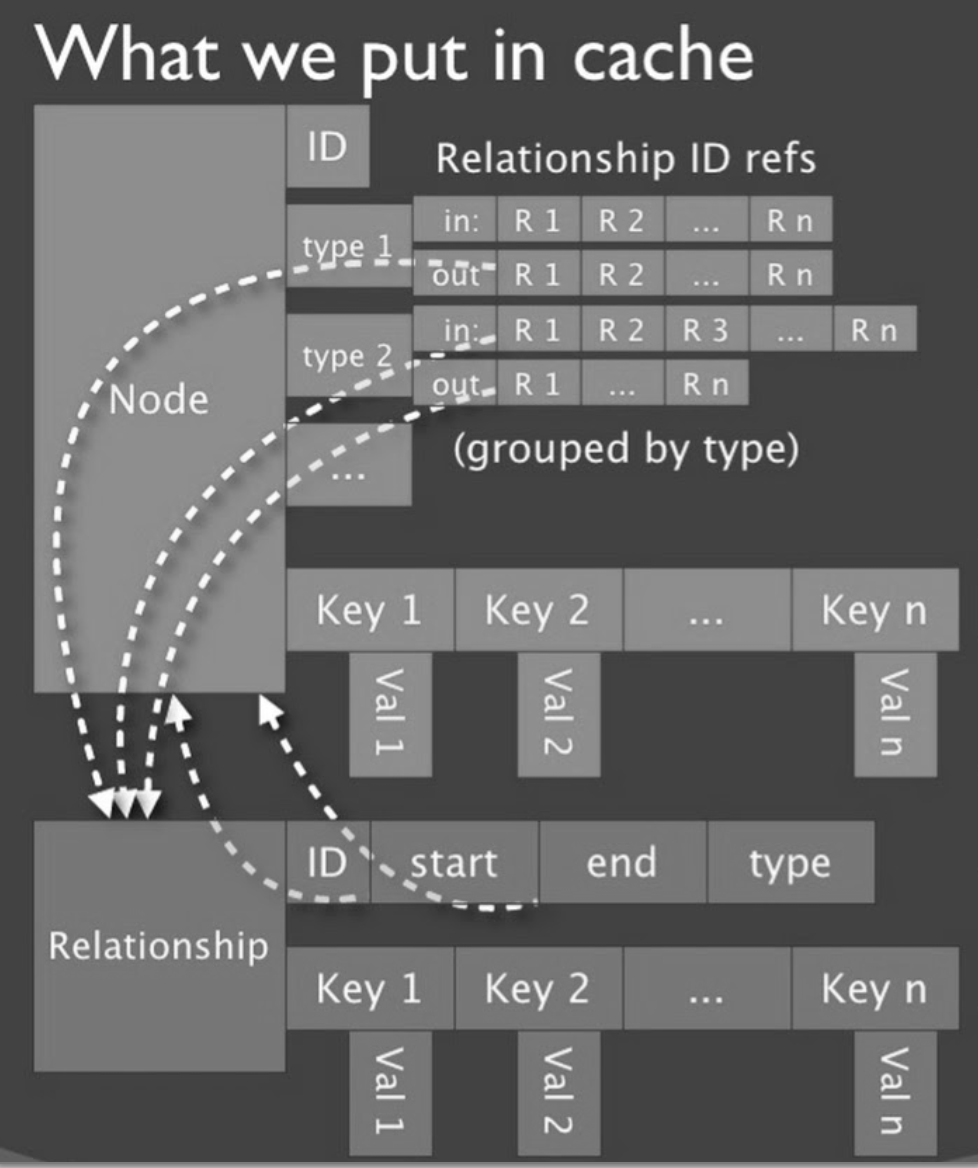
\includegraphics[width=150px, keepaspectratio]{Dokumentation-main-2/main_document/chapters/05-Interaktion-Abgeord/image21.png}
    \caption{Datenorganisation in Graphdatenbanken - Beispiel Neo4j} \cite{generalStorage}
    \label{fig:Dokumentation-main-2/main_document/chapters/05-Interaktion-Abgeord/image21.png}
\end{figure}
Wichtig ist an dieser Darstellung, dass Nodes ihre Relationships zweifach gruppiert speichern \cite{neo4jrelationshipgrouping}. Einerseits werden die Relationships gruppiert nach ihrem Namen (auch Typ) gespeichert. Andererseits wird innerhalb jeder dieser Gruppen differenziert zwischen eingehenden- und ausgehenden Relationships. Durch diese zweifache Gruppierung sollten unter anderem Performanceeinbußen durch Inselbildung nach Typ der Relation oder nach Richtung der Relation vernachlässigbar sein. So muss beispielsweise nicht durch alle eingehenden Relationships iteriert werden, wenn man lediglich nach Ausgehenden sucht.
\subsection{Graphdatenbankschema: Entwurf}
Der Entwurf eines Graphdatenbankschemas ist von einigen Faktoren, u.a. Technischen und Inhaltlichen, abhängig. Diese werden folgend hervorgehoben und definieren eine Art Ausgangslage.
\newline
Die Datenbasis ist insofern für die aktuelle Aufgabenstellung wichtig, als das ohne Verständnis für die bestehenden Datenfelder, das Modellieren eines neuen Modells mit neuen Datenfeldern schwierig ist. Ein Überblick über das Schema wird in der Ausarbeitung von Gruppe 2 gegeben.
Außerdem ist die These des Projektes zu beachten. Es ist somit darauf zu achten, dass gerade Fragestellungen, die eben in Richtung dieser These gehen, angemessen gut abfragbar sein müssen.
\newline
Abschließend werden die konkreten Fragestellungen, die an die Graphdatenbank gestellt werden sollen mit den entsprechenden Verantwortlichen ermittelt. Zum Zeitpunkt der Ermittlung, soll beispielsweise zu einigen Eigenschaften ein \enquote{Score} berechnet werden, wie zum Sender, die viele Nachrichten mit positivem Sentiment verschicken \cite{initialQuestionsGroup7}. Diese \enquote{Scores} sollen (teilweise) für jeweilige Zeitabschnitte berechnet werden, beispielsweise pro Monat. Dies ist insofern relevant, als dass gerade zeitliche Abschnitte vermutlich eine entscheidende Rolle einnehmen.
\newline
Ein erster, eher umfangreicher, Entwurf ist in Abbildung \ref{fig:Dokumentation-main-2/main_document/chapters/05-Interaktion-Abgeord/image8.png} zu sehen. Dieser und folgende Entwürfe wurden nach eigenem Ermessen strukturiert, wobei sich teilweise an Roy-Hubara et al. \cite{graphdatabasemodelling} orientiert wurde.
\begin{figure}[hbt!]
    \centering
    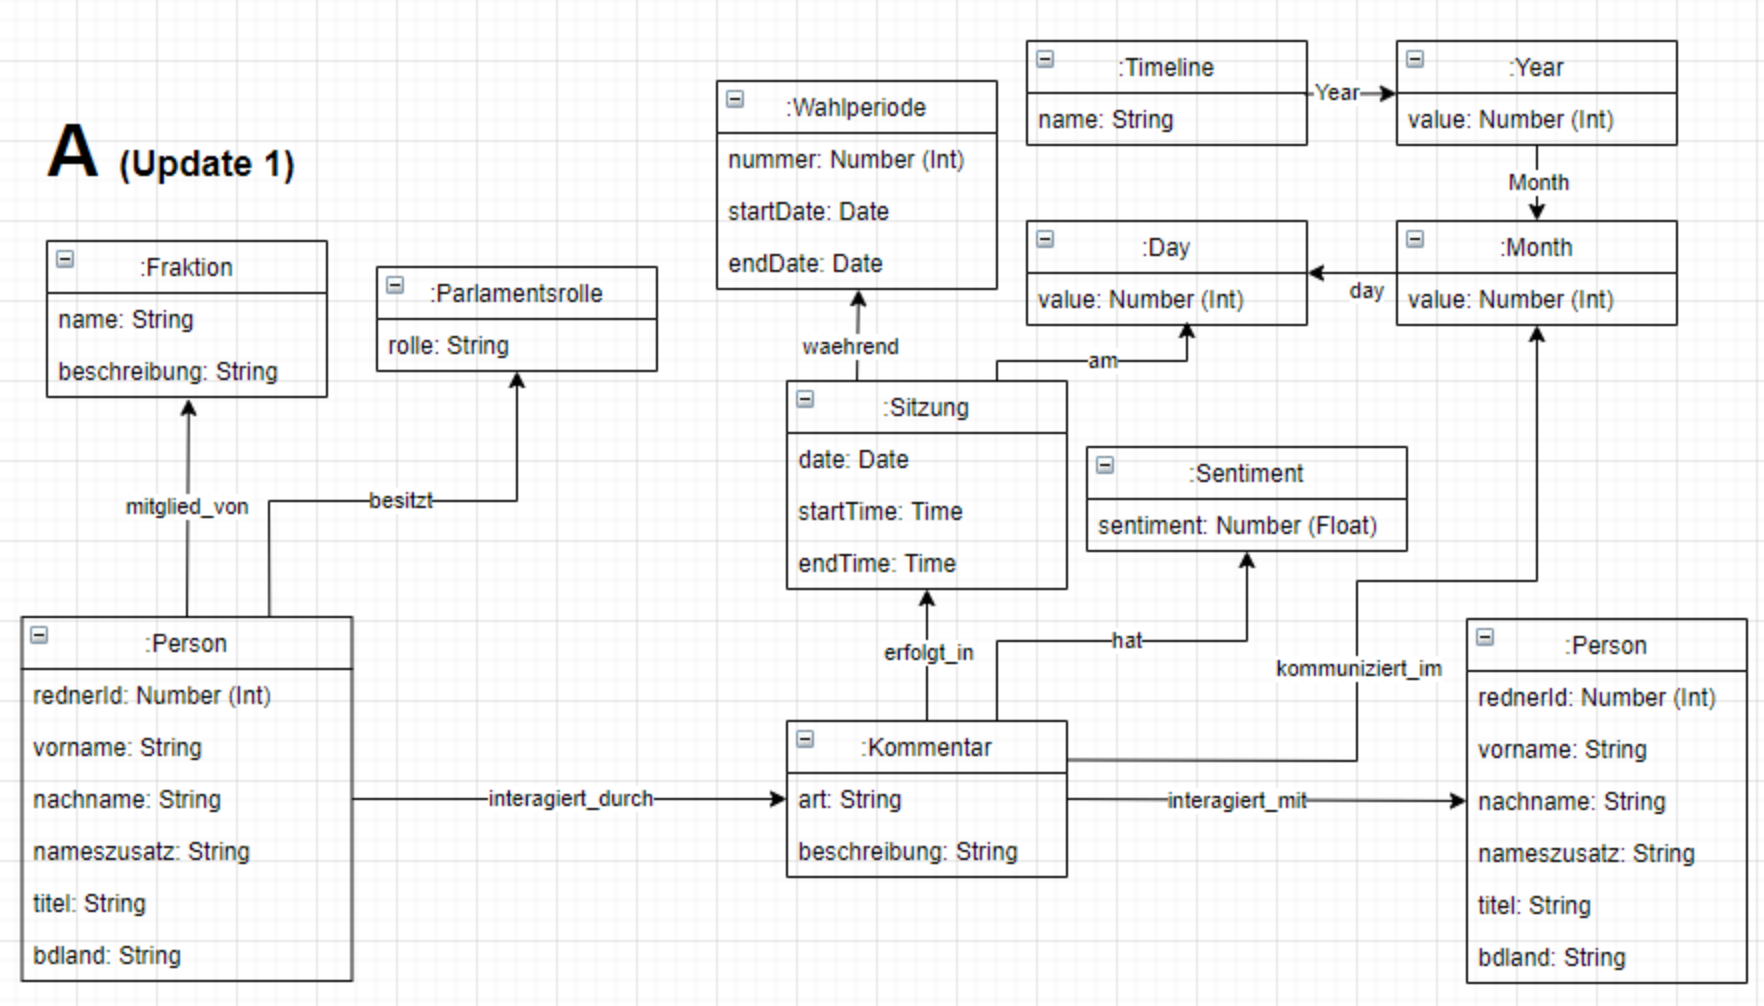
\includegraphics[width=375px, keepaspectratio]{Dokumentation-main-2/main_document/chapters/05-Interaktion-Abgeord/image8.png}
    \caption{Initialer Entwurf Graphdatenbankschema}
    \label{fig:Dokumentation-main-2/main_document/chapters/05-Interaktion-Abgeord/image8.png}
\end{figure}
Der Grafik sind besonders drei Kernüberlegungen zu entnehmen. Innerhalb der Hauptstruktur hat eine Person eine oder mehrere Fraktionen und eine oder mehrere Parlamentsrollen. Die zweite Kernüberlegung ist die Einführung eines sogenannten \enquote{Timeline trees} (TLT) \cite{robinson2015graph} der mit der Sitzung und den jeweiligen Kommentaren verbunden ist. Er verfügt über die Stufen \enquote{:Year}, \enquote{:Month} und \enquote{:Day}. Grund für die Integration ist das Wissen über die Wichtigkeit des Faktors Zeit für die Folgeanalysen. Ohne besagten TLT wäre eine Laufzeit von O(N) zu erreichen. Mit Wissen zu TLT könnte man diese Struktur ausnutzen, um die Zugriffszeit für den Erhalt einer gefilterten Menge deutlich zu erhöhen. Beispielsweise könnte man den Zugriff auf alle Kommentare des Monats Februar im Jahr 2020 von O(N) auf in etwa O(2) durch den Zugriff 2020:Year $\rightarrow$ Februar:Month optimieren.
\newline
Eine dritte Kernüberlegung besteht darin, das Sentiment als externen Knoten aus dem Knoten Kommentar zu extrahieren. Wenn man das eher stetige Sentiment (z.B. 0,34216754) in ein eher diskretes Sentiment (z.B. 0,34) transformiert, ist ein Vorteil bei dem Filtern nach einem bestimmten Sentiment erkennbar (Das Sentiment bewegt sich im Bereich [-1.0, 1.0]). Da diese Transformation bei der Umwandlung der Daten aus der NoSQL-Datenbank in die Neo4j sehr gut möglich ist, sollte diese Überlegung nicht unbemerkt gelassen werden. Da hier beispielsweise nun auf zwei Dezimalstellen nach dem Komma gerundet wurde und das Sentiment sich im Bereich [-1.0, 1.0] bewegt, existieren so 200 verschiedene Gruppen, beziehungsweise demzufolge 200 verschiedene Knotentypen. Der Vorteil wird an einem Beispiel demonstriert. Möchte man eine Menge von Kommentaren erhalten, deren Sentiment positiv ist, müsste man bisher über alle Kommentare iterieren (ca. 70000-250000). Mit der soeben vorgestellten Methode würden sich diese Iterationen auf 100 reduzieren (alle 100 positiven Sentiment-Knoten z.B. 0.01, 0.02, 0.03, ...). Der Basisentwurf ist in Abbildung \ref{fig:Dokumentation-main-2/main_document/chapters/05-Interaktion-Abgeord/image9.png} dargestellt.
\begin{figure}[htb]
    \centering
    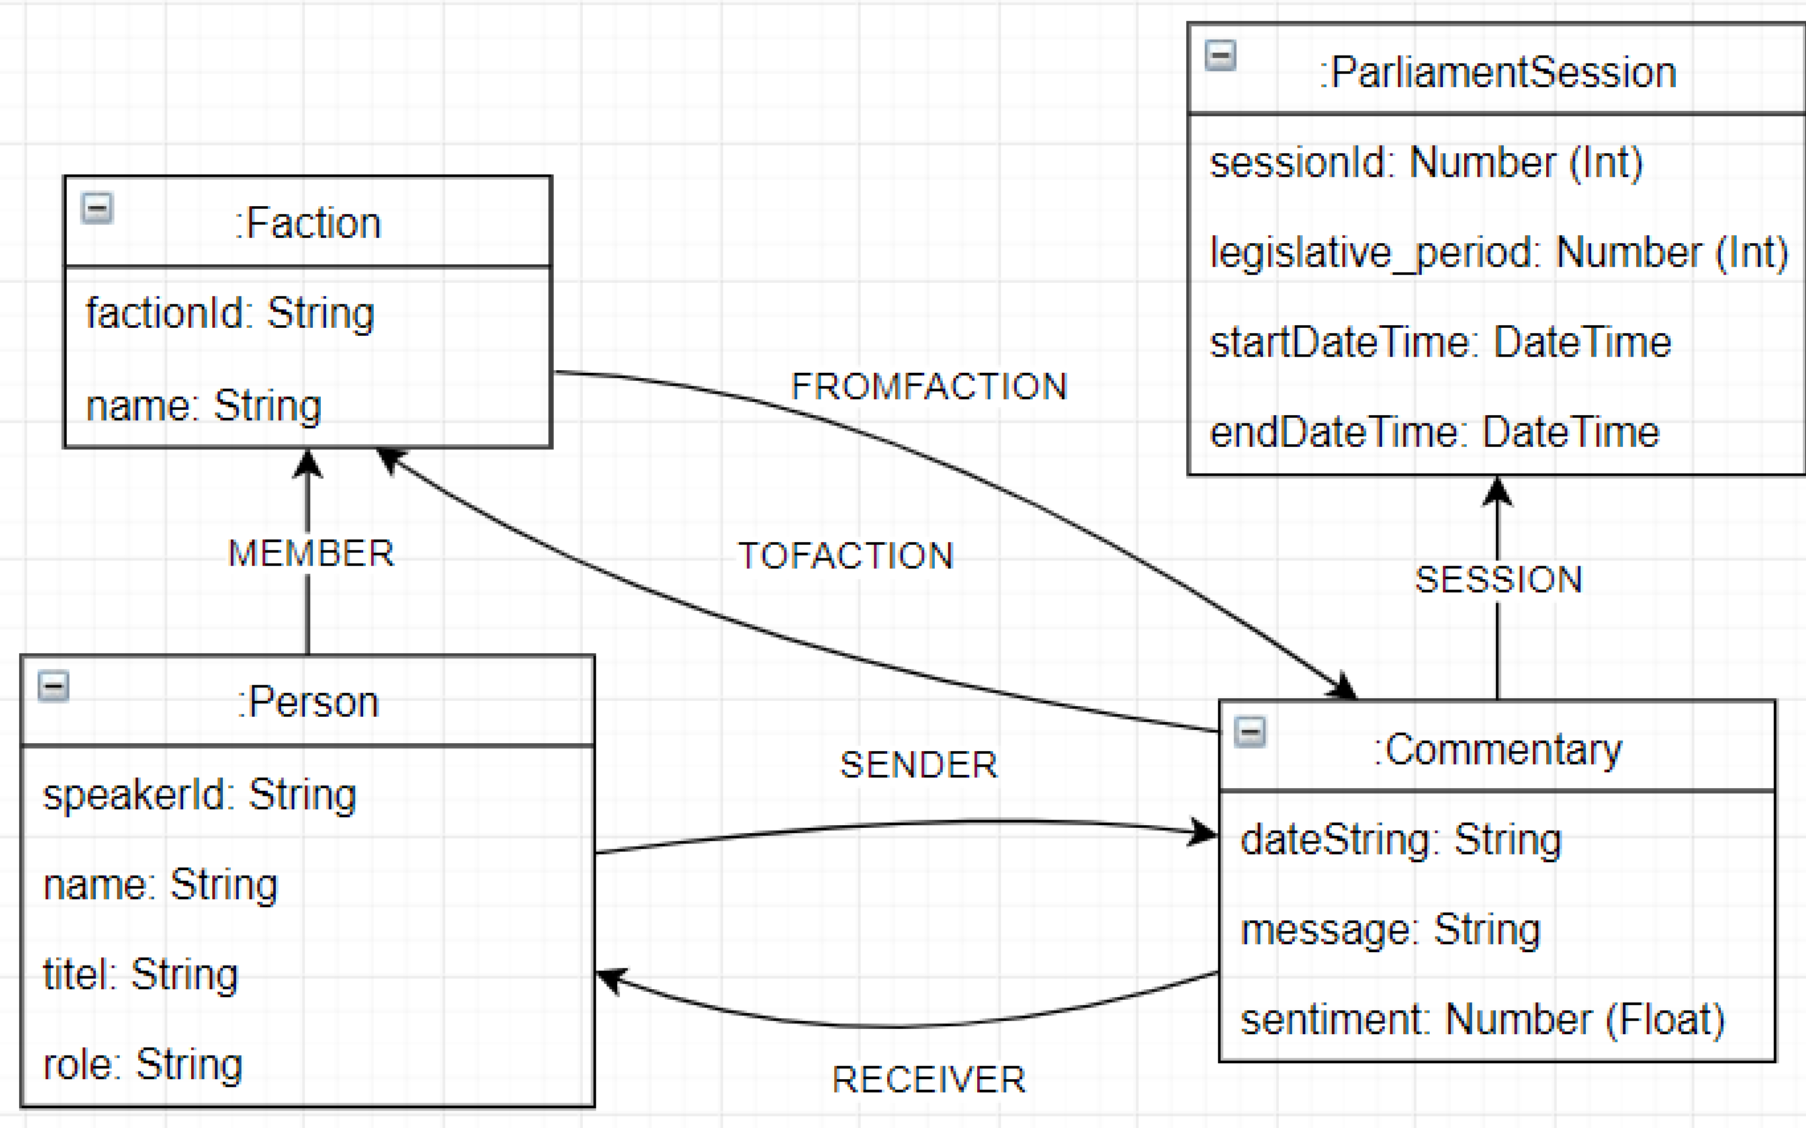
\includegraphics[width=250px]{Dokumentation-main-2/main_document/chapters/05-Interaktion-Abgeord/diagramm.png} 
    \caption{Datenbankschema}
    \label{fig:Dokumentation-main-2/main_document/chapters/05-Interaktion-Abgeord/image9.png}
\end{figure}
Innerhalb der Hauptstruktur ist erkennbar, dass nun zwischen Knoten mit dem Label \enquote{:Commentary} und \enquote{:Faction} eine eingehende- und eine ausgehende Relationship hinzugefügt wurde. Der Grund dafür ist, dass nun teilweise Interaktionen zwischen einem Abgeordneten (einer Person) und einer Partei als Gesamtes identifiziert wurden. Darüber hinaus wurde auf den TLT verzichtet. Grund dafür war, dass dieser anscheinend schwieriger umzusetzen ist.
\section{Umsetzung}\label{sec:04_03_umsetzung}
(Autor: Rico Stucke)
\subsection{Lesen aus MongoDB}
Zunächst haben wir uns mit dem Empfang der Daten aus der MongoDB von Team 3 beschäftigt. Für die Abfrage der Daten aus der MongoDB benutzen wir die pymongo Library von Python. Der Client öffnet eine Verbindung zur Datenbank von Gruppe 3 und liest alle Collections, die sich in der Datenbank befinden. Jede Collection entspricht dabei einem Sitzungstag. Im nächsten Schritt aggregieren wir alle ausgelesenen Werte, formen diese um und entfernen eventuelle Dopplungen, die vor allem bei wiederkehrenden Personen oder Fraktionen auftreten. Am Ende dieses Prozesses entstehen Dictionaries, die alle einzigartigen Personen und Fraktionen, sowie Sitzungstage und Kommentare, beinhalten.
\subsection{Nodes \& Relations}
Mit der neomodel Library, die als Object Graph Mapper dient, können Klassen definiert werden, die dann von neomodel als Knoten in Neo4j übernommen werden. Außerdem können an diesen Klassen auch die Beziehungen zwischen den Klassen definiert werden. Die entstandenen Dictionaries dienen als Datengrundlage für die Knotenklassen in neomodel.
\begin{figure}[htb]
    \centering
    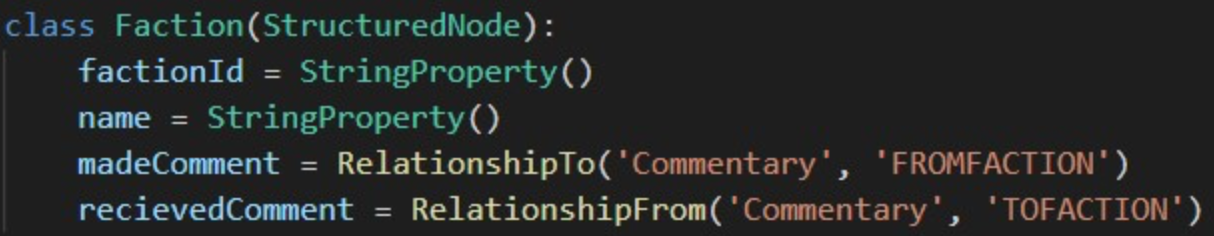
\includegraphics[width=10cm]{Dokumentation-main-2/main_document/chapters/05-Interaktion-Abgeord/faction.jpg} 
    \caption{Beispiel einer neomodel Klasse}
    \label{fig:commentary}
\end{figure}
Abbildung 5 zeigt beispielhaft eine Klasse aus dem Programm, um zu verdeutlichen wie neomodel verwendet wird, um einen Node in der Datenbank zu definieren. Durch die Implementierung von StructuredNode wird neomodel mitgeteilt, dass eine Klasse ein Node in der Datenbank sein soll und über die RelationshipTo und RelationshipFrom Funktionen können die Relationen definiert werden, die von diesem Knoten ausgehen oder eingehen.
\subsection{Neo4j DB Connection}
Die Python library neomodel bietet für das Erzeugen von Nodes und Relations in Neo4j ein einfaches Interface, dass durch seine StructuredNode-Klasse implementiert wird. Dadurch wird es möglich einen Node, der durch eine Klasse, die StructuredNode implementiert, dargestellt wird, über zwei Funktionen in der Datenbank zu speichern und Relationen mit anderen Node-Klassen aufzubauen.\\
Das Speichern Erfolg durch die von StructuredNode geerbte Methode save(). Hierbei sind keine weiteren Angaben nötig. Diese Methode muss nur vom jeweilig instanziierten Objekt aufgerufen werden, um es in die Datenbank zu übertragen. Für die Herstellung einer Relation muss die connect()-Methode aufgerufen werden. Wichtig hierbei ist, dass die Klasse ein Attribut mit dem Namen der Relation implementieren muss. Der Funktionsaufruf erfolgt dann in dem folgenden Schema:\\
\newcommand\tab[1][1cm]{\hspace*{#1}}
\tab ObjektA.relation\_name.connect(ObjektB)
\subsection{Laufzeitverbesserungen}
In seiner ersten Iteration hat das Programm für die Übertragung einer Collection aus MongoDB in die Neo4jDB rund 5 Minuten gebraucht. Da eine Collection aber nur einen Sitzungstag umfasst, wurde schnell klar, dass Verbesserungen an der Laufzeit nötig sind. Durch Änderungen am Code konnte die Geschwindigkeit gesteigert werden indem nicht mehr für jede Datenbankaktion eine Transaktion verwendet wird, sondern mehrere Aktionen gebündelt werden in einer Transaktion.\\
Bei einem Test mit einer lokalen Neo4j Datenbank, die außerhalb des HTW-Netzes lief, konnte auch beobachtet werden, dass das Programm wesentlich schneller läuft. Hierbei handelte es sich um Differenzen von 8 Schreibaktionen in der Datenbank pro Sekunde, wenn das Programm von einem privaten Rechner gestartet wurde, der über einen Tunnel mit dem HTW-Netz verbunden war, zu über 200 Schreibaktionen wenn das Programm auf dem selben Rechner lief, der auch die Datenbank gehostet hat. Diese Beobachtung führte dann dazu, dass das Programm um eine einfache REST-API und einen simplen Flask-Server erweitert wurde. Dies ermöglichte es das Programm direkt auf der Hardware laufen zu lassen, die auch die Neo4j Datenbank enthält im HTW-Netz. Durch diese Änderungen gelang es uns die Laufzeit von ursprünglich geschätzten 13 Stunden auf rund 25 Minuten zu reduzieren.
\section{Ergebnisse}\label{sec:04_04_ergebnisse}
(Autoren: Jennifer Vormann | Rico Stucke)\\
\\
In seiner jetzigen Form erzeugt das Skript die Neo4j Datenbank in 25 Minuten. Dabei werden rund 278000 Knoten und 830000 Beziehungen zwischen diesen Knoten angelegt. Den größten Anteil dabei haben mit rund 276000 Knoten die Kommentare der Abgeordneten und Fraktionen. Die lange Laufzeit des Programms lässt sich erklären durch das Fehlen eines Batch-Prozesses für die Inserts in die Datenbank. Neomodel bietet zwar eine Möglichkeit für Batch-Inserts, aber es besteht dabei keine Möglichkeit gleichzeitig die Beziehungen mit anzulegen.\\
\begin{figure}[htb]
    \centering
    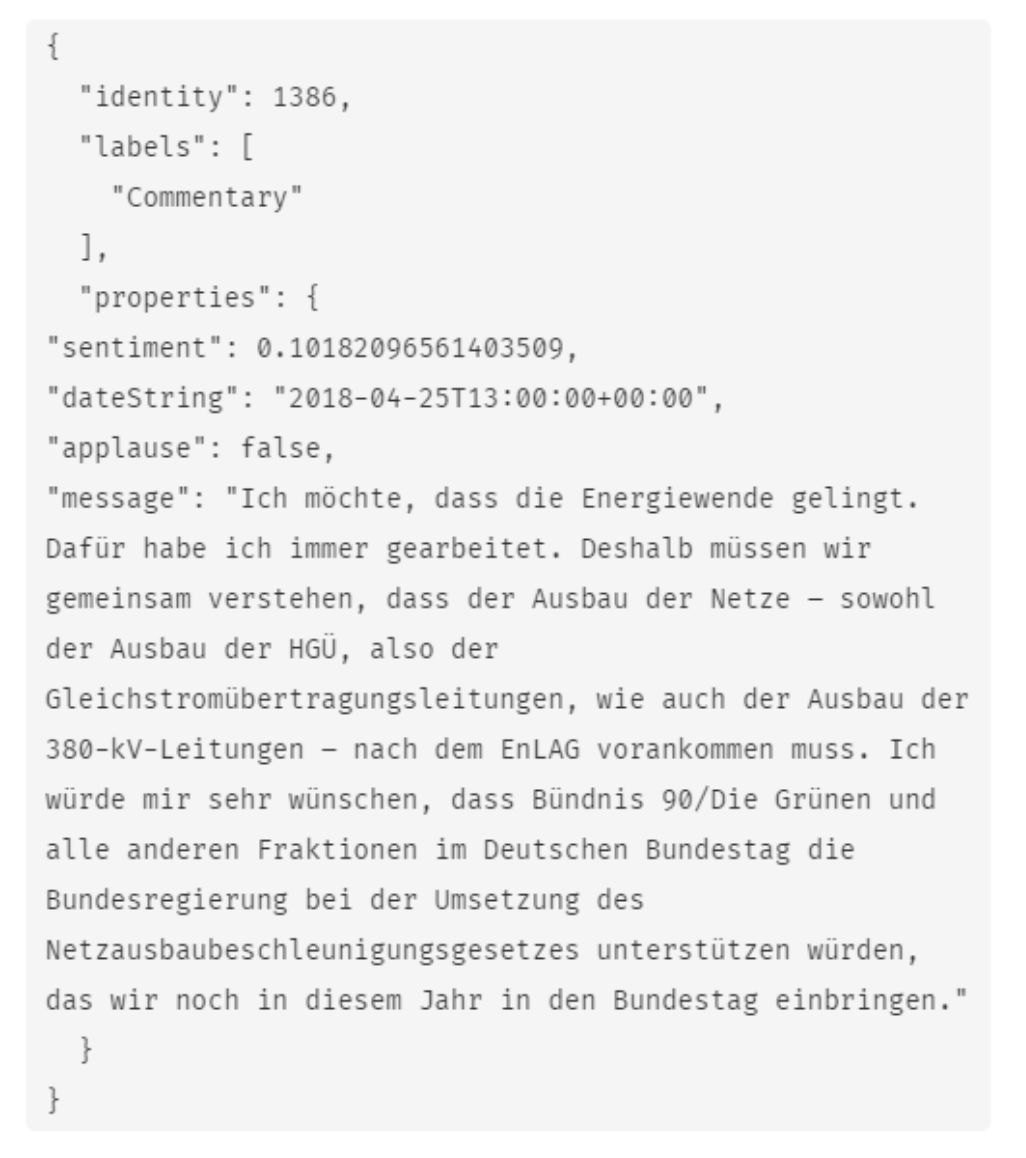
\includegraphics[width=8cm]{Dokumentation-main-2/main_document/chapters/05-Interaktion-Abgeord/5.PNG} 
    \caption{Ausgabe eines Kommentars}
    \label{fig:commentary}
\end{figure}
Ein weiteres Ergebnis und deren Visualisierung zeigt die Abbildung der Personen und des Sendens eines Kommentars in Richtung einer anderen Person oder Fraktion. Wir haben uns für die Darstellung dieses Graphen in die Dokumentation entschieden, weil der Fokus der Arbeit auf den Kommentare und deren Sentiments liegt. Die Graphen, die in Neo4j angezeigt werden können, sind schnell sehr komplex und können nur in kleinen Mengen (default: 300 Nodes) dargestellt werden.
\begin{figure}[htb]
    \centering
    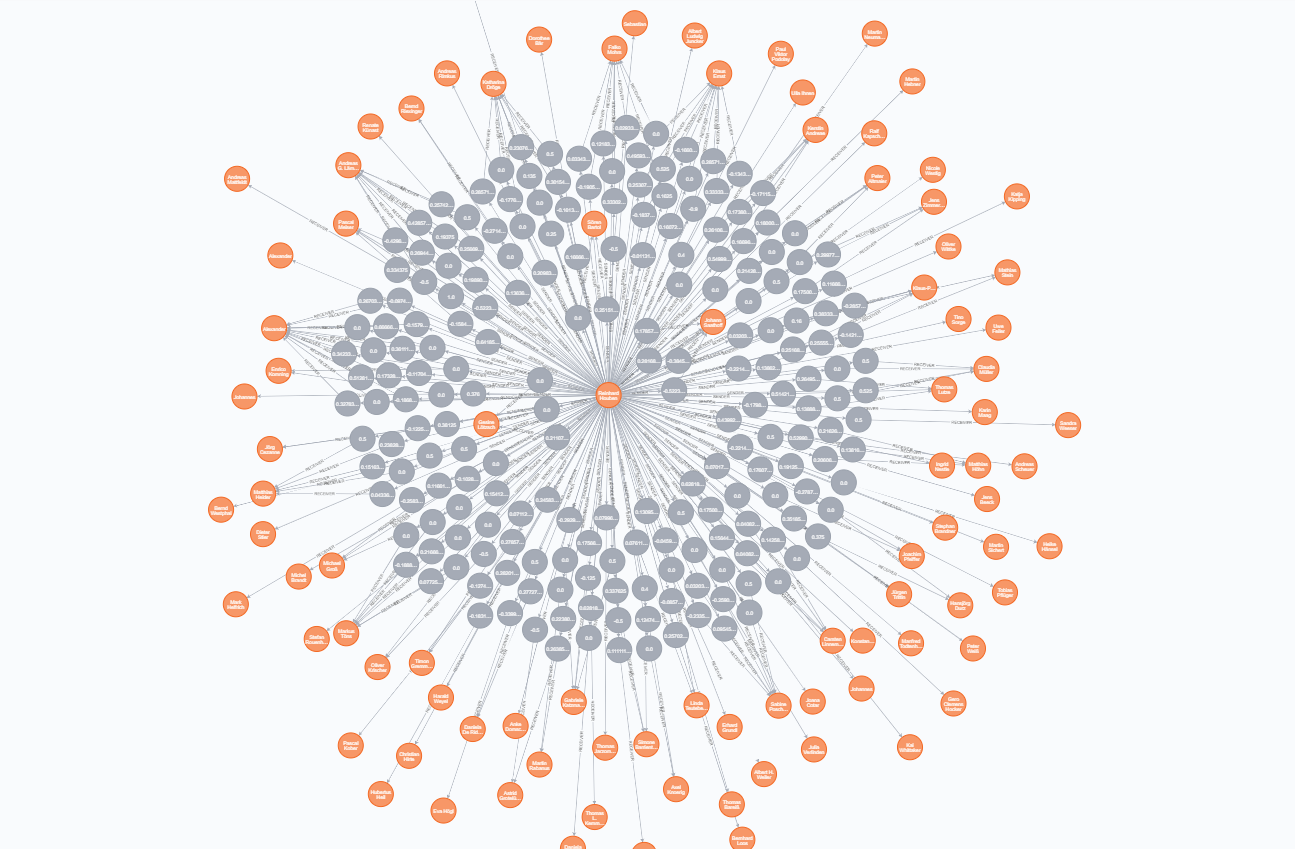
\includegraphics[width=\textwidth]{Dokumentation-main-2/main_document/chapters/05-Interaktion-Abgeord/6.PNG} 
    \caption{Neo4J Graph -> Person - Sender - Commentary - Receiver - Person}
    \label{fig:personcomment}
\end{figure}
\section{Ausblick}\label{sec:04_05_ausblick}
(Autoren: Jennifer Vormann | Florian Thom)\\
\\
Künftig wäre es eines unserer Ziele, die Laufzeit der Anwendung zu verbessern. Hierzu könnte generell noch einmal über den Code gegangen und dieser optimiert werden. So könnte die Runtime gegebenenfalls verbessert werden, um schnelles Schreiben in die Graphdatenbank zu ermöglichen. 
Zusammenfassend können folgende Punkte für eine Weiterentwicklung analysiert und gegebenenfalls umgesetzt werden:\\
- Arbeiten mit Batch\\
- Libraries | Programmiersprache variieren \\
\\
Ebenso wäre es ein Anliegen, die weiteren Wahlperioden zu ergänzen. Bei Optimierungen des Codes würden wir aller Wahrscheinlichkeit nach auf die Verwendung von neomodel verzichten und auf die Standard Implementierung mit Neo4j Python Driver ausweichen. Bei der Erweiterung um andere Wahlperioden wäre zu überdenken, die Wahlperiode als eigenen Node zu erstellen. Dazu müsste das Datenbankschema entsprechend angepasst werden.\\
Gerade im Entwurf wurden gewisse Optimierungen vorgestellt, bei denen aus theoretischer Sicht teilweise gute Verbesserungsmöglichkeiten gesehen wurden. Anfänglich wurde über einen praktischen Test oder Vergleich der Schemata spekuliert. Dieser Test blieb leider aufgrund von gewissen Schwierigkeiten in der Implementierung aus und könnte perspektivisch noch durchgeführt werden. Verbesserungsmöglichkeiten sind aus unserer Perspektive bezüglich des finalen Entwurfes vorhanden. Diese bestehen besonders in der Einbindung eines TLTs. Dies wurde mit dem ersten Entwurf aus theoretischer Sicht erläutert.
\section{Lernziele}\label{sec:04_07_lernziele}
(Autorin: Jennifer Vormann)\\
\\
Die Lernziele dieses Projektes und des damit verbundenen Kurses waren sehr vielfältig. In den Vorlesungen wurde Grundlagenwissen in den folgenden Bereichen vermittelt:\\
- Informationssysteme allgemein \& Dateninspektion\\
- Crawling Textanalyse \& NoSQL\\
- Sentiment Analyse \& Graphdatenbanken\\
\\
Aufgrund der Art der Durchführung der Übungen konnte das Format der Plenarsitzungen, inklusive deren Rollen, erlernt werden. Das Einsetzen realer Daten und deren Verarbeitung gehört zu den erreichten Lernzielen, ebenso wie das Extrahieren der relevanten Informationen aus den gegebenen Daten. Die Daten mussten betrachtet und bewertet werden anhand ihrer Relevanz für das Ziel der gesamten Projektaufgabe. Anschließend wurde das Aggregieren, Verknüpfen und Darstellen der Daten erlernt.\\
Zur Erstellung des Datenbankschemas wurden Kenntnisse zu Klassendiagrammen in Notation der UML vertieft und angewandt. Für die Zwischen- und Abschlusspräsentation der Vorgehensweise, konnte unser Wissen über das Schreiben eines Proof of Concept und das ansprechende Erstellen von Präsentationen gefestigt werden. Wir haben den Umgang mit Neo4j und deren deklarative Abfragesprache Cypher neu erlernt. Bei der Verarbeitung der Daten die von Gruppe 3 geliefert wurden und beim Weiterleiten unserer Ergebnisse an Gruppe 7 haben wir erfolgreich Schnittstellen von verschiedenen Datenbanken hergestellt. Unser Vorgehen und die Wahl der Technologien für die gesamte Umsetzung unserer Teilaufgabe lagen komplett in unserer Hand. Daher mussten wir abwägen, recherchieren und Vor- und Nachteile evaluieren. Die Kommunikation und Kollaboration war nicht nur in unserem Team wichtig sondern auch teamübergreifend. Auch das Verfassen einer kursumfassenden Dokumentation benötigte ein merklich höheres Maß an Abstimmung, Organisation und Kommunikation. Eigenständiges Arbeiten und Praktiken des Zeitmanagements konnten festigen werden.
